\documentclass[a4paper,twoside]{article}
% My LaTeX preamble file - by Nathaniel Dene Hoffman
% Credit for much of this goes to Olivier Pieters (https://olivierpieters.be/tags/latex)
% and Gilles Castel (https://castel.dev)
% There are still some things to be done:
% 1. Update math commands using mathtools package (remove ddfrac command and just override)
% 2. Maybe abbreviate \imath somehow?
% 3. Possibly format for margin notes and set new margin sizes
% First, some encoding packages and useful formatting
%--------------------------------------------------------------------------------------------
\usepackage{import}
\usepackage{pdfpages}
\usepackage{transparent}
\usepackage[l2tabu,orthodox]{nag}   % force newer (and safer) LaTeX commands
\usepackage[utf8]{inputenc}         % set character set to support some UTF-8
                                    %   (unicode). Do NOT use this with
                                    %   XeTeX/LuaTeX!
\usepackage[T1]{fontenc}
\usepackage[english]{babel}         % multi-language support
\usepackage{sectsty}                % allow redefinition of section command formatting
\usepackage{tabularx}               % more table options
\usepackage{booktabs}
\usepackage{titling}                % allow redefinition of title formatting
\usepackage{imakeidx}               % create and index of words
\usepackage{xcolor}                 % more colour options
\usepackage{enumitem}               % more list formatting options
\usepackage{tocloft}                % redefine table of contents, new list like objects
\usepackage{subfiles}               % allow for multifile documents

% Next, let's deal with the whitespaces and margins
%--------------------------------------------------------------------------------------------
\usepackage[centering,margin=1in]{geometry}
\setlength{\parindent}{0cm}
\setlength{\parskip}{2ex plus 0.5ex minus 0.2ex} % whitespace between paragraphs

% Redefine \maketitle command with nicer formatting
%--------------------------------------------------------------------------------------------
\pretitle{
  \begin{flushright}         % align text to right
    \fontsize{40}{60}        % set font size and whitespace
    \usefont{OT1}{phv}{b}{n} % change the font to bold (b), normally shaped (n)
                             %   Helvetica (phv)
    \selectfont              % force LaTeX to search for metric in its mapping
                             %   corresponding to the above font size definition
}
\posttitle{
  \par                       % end paragraph
  \end{flushright}           % end right align
  \vskip 0.5em               % add vertical spacing of 0.5em
}
\preauthor{
  \begin{flushright}
    \large                   % font size
    \lineskip 0.5em          % inter line spacing
    \usefont{OT1}{phv}{m}{n}
}
\postauthor{
  \par
  \end{flushright}
}
\predate{
  \begin{flushright}
  \large
  \lineskip 0.5em
  \usefont{OT1}{phv}{m}{n}
}
\postdate{
  \par
  \end{flushright}
}

% Mathematics Packages
\usepackage[Gray,squaren,thinqspace,cdot]{SIunits}      % elegant units
\usepackage{amsmath}                                    % extensive math options
\usepackage{amsfonts}                                   % special math fonts
\usepackage{mathtools}                                  % useful formatting commands
\usepackage{amsthm}                                     % useful commands for building theorem environments
\usepackage{amssymb}                                    % lots of special math symbols
\usepackage{mathrsfs}                                   % fancy scripts letters
\usepackage{cancel}                                     % cancel lines in math
\usepackage{esint}                                      % fancy integral symbols
\usepackage{relsize}                                    % make math things bigger or smaller
%\usepackage{bm}                                         % bold math!
\usepackage{slashed}

\newcommand\ddfrac[2]{\frac{\displaystyle #1}{\displaystyle #2}}    % elegant fraction formatting
\allowdisplaybreaks[1]                                              % allow align environments to break on pages

% Ensure numbering is section-specific
%--------------------------------------------------------------------------------------------
\numberwithin{equation}{section}
\numberwithin{figure}{section}
\numberwithin{table}{section}

% Citations, references, and annotations
%--------------------------------------------------------------------------------------------
\usepackage[small,bf,hang]{caption}        % captions
\usepackage{subcaption}                    % adds subfigure & subcaption
\usepackage{sidecap}                       % adds side captions
\usepackage{hyperref}                      % add hyperlinks to references
\usepackage[noabbrev,nameinlink]{cleveref} % better references than default \ref
\usepackage{autonum}                       % only number referenced equations
\usepackage{url}                           % urls
\usepackage{cite}                          % well formed numeric citations
% format hyperlinks
\colorlet{linkcolour}{black}
\colorlet{urlcolour}{blue}
\hypersetup{colorlinks=true,
            linkcolor=linkcolour,
            citecolor=linkcolour,
            urlcolor=urlcolour}

% Plotting and Figures
%--------------------------------------------------------------------------------------------
\usepackage{tikz}          % advanced vector graphics
\usepackage{pgfplots}      % data plotting
\usepackage{pgfplotstable} % table plotting
\usepackage{placeins}      % display floats in correct sections
\usepackage{graphicx}      % include external graphics
\usepackage{longtable}     % process long tables

% use most recent version of pgfplots
\pgfplotsset{compat=newest}

% Misc.
%--------------------------------------------------------------------------------------------
\usepackage{todonotes}  % add to do notes
\usepackage{epstopdf}   % process eps-images
\usepackage{float}      % floats
\usepackage{stmaryrd}   % some more nice symbols
\usepackage{emptypage}  % suppress page numbers on empty pages
\usepackage{multicol}   % use this for creating pages with multiple columns
\usepackage{etoolbox}   % adds tags for environment endings
\usepackage{tcolorbox}  % pretty colored boxes!


% Custom Commands
%--------------------------------------------------------------------------------------------
\newcommand\hr{\noindent\rule[0.5ex]{\linewidth}{0.5pt}}                % horizontal line
\newcommand\N{\ensuremath{\mathbb{N}}}                                  % blackboard set characters
\newcommand\R{\ensuremath{\mathbb{R}}}
\newcommand\Z{\ensuremath{\mathbb{Z}}}
\newcommand\Q{\ensuremath{\mathbb{Q}}}
%\newcommand\C{\ensuremath{\mathbb{C}}}
\renewcommand{\arraystretch}{1.2}                                       % More space between table rows (could be 1.3)
\newcommand{\Cov}{\mathrm{Cov}}
\newcommand\D{\mathrm{D}}
\newcommand*{\dbar}{\ensuremath{\text{\dj}}}

\newcommand{\incfig}[2][1]{%
    \def\svgwidth{#1\columnwidth}
    \import{./figures/}{#2.pdf_tex}
}

% Custom Environments
%--------------------------------------------------------------------------------------------
\newcommand{\lecture}[3]{\hr\\{\centering{\large\textsc{Lecture #1: #3}}\\#2\\}\hr\markboth{Lecture #1: #3}{\rightmark}}   % command to title lectures
\usepackage{mdframed}
\theoremstyle{plain}
\newmdtheoremenv[nobreak]{theorem}{Theorem}[section]
\newtheorem{corollary}{Corollary}[theorem]
\newtheorem{lemma}[theorem]{Lemma}
\theoremstyle{definition}
\newtheorem*{ex}{Example}
\newmdtheoremenv[nobreak]{definition}{Definition}[section]
\theoremstyle{remark}
\newtheorem*{remark}{Remark}
\newtheorem*{claim}{Claim}
\AtEndEnvironment{ex}{\null\hfill$\diamond$}%
% Note: A proof environment is already provided in the amsthm package
\tcbuselibrary{breakable}
\newenvironment{note}[1]{\begin{tcolorbox}[
    arc=0mm,
    colback=white,
    colframe=white!60!black,
    title=#1,
    fonttitle=\sffamily,
    breakable
]}{\end{tcolorbox}}
\newenvironment{problem}{\begin{tcolorbox}[
    arc=0mm,
    breakable,
    colback=white,
    colframe=black
]}{\end{tcolorbox}}

% Header and Footer
%--------------------------------------------------------------------------------------------
% set header and footer
\usepackage{fancyhdr}                       % header and footer
\pagestyle{fancy}                           % use package
\fancyhf{}
\fancyhead[LE,RO]{\textsl{\rightmark}}      % E for even (left pages), O for odd (right pages)
\fancyfoot[LE,RO]{\thepage}
\fancyfoot[LO,RE]{\textsl{\leftmark}}
\setlength{\headheight}{15pt}


% Physics
%--------------------------------------------------------------------------------------------
\usepackage[arrowdel]{physics}      % all the usual useful physics commands
\usepackage{feyn}                   % for drawing Feynman diagrams
%\usepackage{bohr}                   % for drawing Bohr diagrams
%\usepackage{tikz-feynman}
\usepackage{elements}               % for quickly referencing information of various elements
\usepackage{tensor}                 % for writing tensors and chemical symbols

% Finishing touches
%--------------------------------------------------------------------------------------------
\author{Nathaniel D. Hoffman}

\title{33-755 Homework 9}
\date{\today}
\begin{document}
\maketitle

\section{Schrodinger Equation for Bloch Function}
The time independent Schr\"odinger equation for the Hamiltonian
\begin{equation}
    \vu{H} = \frac{\vu{P}^2}{2m} + V(x),
\end{equation}
with periodic potential $ V(x + a) = V(x) $, has solutions of the form
\begin{equation}
    \varphi(x) = e^{\imath q x} u_q(x)
\end{equation}
where $ u_q(x + a) = u_q(x) $ is periodic with the same periodicity as $ V $. This function $ u_q(x) $ obeys a Schr\"odinger equation with Hamiltonian $ H_q $ that depends on the Bloch index $ q $. Determine $ H_q $.

\begin{problem}
    We can solve this problem by plugging the solution into the Schr\"odinger equation:
    \begin{align}
        \vu{H} e^{\imath q x} u_q(x) &= - \frac{\hbar^2}{2 m} \partial_x^2 e^{\imath q x} u_q(x) + V(r) e^{\imath q x} u_q(x) \\
        &= - \frac{\hbar^2}{2m} \left( - e^{\imath q x} q^2 u_q(x) + 2 \imath q e^{\imath q x} \partial_x u_q(x) + e^{\imath q x} \partial_x^2 u_q(x) \right) + V(r) e^{\imath q x} u_q(x)
    \end{align}
    Dividing out the exponential, we find the following equation for $ u_q(x) $:
    \begin{equation}
        H_q u_q(x) = \left( \frac{\hbar^2 q^2}{2m} + V(r) \right) u_q(x) - \frac{\imath \hbar^2 q}{m} \partial_x u_q(x) - \frac{\hbar^2}{2m} \partial_x^2 u_q(x)
    \end{equation}
    Writing this in terms of momentum operators, we find:
    \begin{equation}
        \vu{H}_q = \frac{\hbar q \vu{P}}{m} + \frac{\vu{P}^2}{2m} + \left( V(r) + \frac{\hbar^2 q^2}{2m} \right)
    \end{equation}
\end{problem}

\section{The Kronig-Penney Model}
The Kronig-Penney model is a model for electrons in crystalline solids. The square wells have width $ a $ and height $ V_0 $, and are placed periodically at intervals $ L $, extending to $ \pm \infty $. An electron of mass $ m $  and energy $ E $ is present.
\begin{itemize}
    \item[(a)] Determine the matrix $ M $ that relates the coefficients of plane waves $ e^{\pm \imath kx} $ in one valley (region where $ V(x) = 0 $) to the next.
        \begin{problem}
            I will set up our potential as follows:
            \begin{equation}
                V =
                \begin{cases}
                    0 & x < - \frac{a}{2} \\
                    V_0 & - \frac{a}{2} < x < \frac{a}{2} \\
                    0 & \frac{a}{2} < x
                \end{cases}
            \end{equation}
            In these regions, the wave function can be described as
            \begin{equation}
                \psi(x) =
                \begin{cases}
                    A e^{\imath k x} + B e^{- \imath k x} & x < - \frac{a}{2} \\
                    C e^{\imath k' x} + D e^{- \imath k' x} & - \frac{a}{2} < x < \frac{a}{2} \\
                    F e^{\imath k x} + G e^{- \imath k x} & \frac{a}{2} < x
                \end{cases}
            \end{equation}
            where $ k = \sqrt{\frac{2mE}{\hbar^2}} $ and $ k' = \sqrt{\frac{2m(E-V_0)}{\hbar^2}} $.

            Let's first compute the matching conditions at $ x = - \frac{a}{2} $. Continuity of the wave function implies
            \begin{equation}
                A e^{-\imath k \frac{a}{2}} + B e^{\imath k \frac{a}{2}} = C e^{-\imath k' \frac{a}{2}} + D e^{\imath k' \frac{a}{2}} 
            \end{equation}
            Continuity of the derivative implies
            \begin{equation}
                k A e^{- \imath k \frac{a}{2}} - k B e^{\imath k \frac{a}{2}} = q C e^{- \imath k' \frac{a}{2}} - q D e^{\imath k' \frac{a}{2}}
            \end{equation}
            We can describe these equations in terms of matrices:
            \begin{equation}
                P \mqty(A \\ B) = Q \mqty(C \\ D) 
            \end{equation}
            where
            \begin{equation}
                P = \mqty(e^{-\imath k \frac{a}{2}} & e^{\imath k \frac{a}{2}} \\ k e^{- \imath k \frac{a}{2}} & - k e^{\imath k \frac{a}{2}})
            \end{equation}
            and
            \begin{equation}
                Q = \mqty(e^{-\imath k' \frac{a}{2}} & e^{\imath k' \frac{a}{2}} \\ k' e^{- \imath k' \frac{a}{2}} & - k' e^{\imath k' \frac{a}{2}})
            \end{equation}
            We see that a transfer matrix is formed from the valley to inside the barrier: $ M = P^{-1} \vdot Q $. We can use time-reversal symmetry to calculate the other half of the transfer function, from the barrier to the next valley.
            \begin{align}
                M &= P^{-1} \vdot Q \vdot (Q^*)^{-1} \vdot P^* \\
                &= \mqty(e^{\imath k a} \left( \cos(k'a) - \imath \frac{(k^2 + k'^2) \sin(k'a)}{2kk'} \right) & \imath \frac{(k^2 - k'^2) \sin(k'a)}{2kk'} \\ - \imath \frac{(k^2 - k'^2) \sin(k'a)}{2kk'} & e^{- \imath ka} \left( \cos(k'a) + \imath \frac{(k^2 + k'^2) \sin(k'a)}{2kk'} \right))
            \end{align}
        \end{problem}
    \item[(b)] What condition must $ M $ satisfy in order for a propagating solution to exist?
        \begin{problem}
            $ M $ can be written as
            \begin{equation}
                M = \mqty(\gamma & \delta^* \\ \delta & \gamma^*)
            \end{equation}
            and
            \begin{equation}
                \mqty(A \\ B) = M \mqty(F \\ G)
            \end{equation}
            To conserve the probability current, we want
            \begin{equation}
                \abs{A}^2 - \abs{B}^2 = \abs{F}^2 - \abs{G}^2
            \end{equation}
            and using the above relation
            \begin{align}
                \abs{F}^2 - \abs{G}^2 &= (\gamma A + \delta^* B)(\gamma^* A^* + \delta B^*) - (\delta A + \gamma^* B)(\delta^* A^* + \gamma B^*) \\
                &= (\abs{\gamma}^2 - \abs{\delta}^2)(\abs{A}^2 - \abs{B}^2)
            \end{align}
            We want these to be equal, so
            \begin{equation}
                \abs{\gamma}^2 - \abs{\delta}^2 = 1
            \end{equation}
            but this is just the determinant of $ M $, so the condition to have a propagating solution is
            \begin{equation}
                \det(M) = 1
            \end{equation}
        \end{problem}
    \item[(c)] Sketch the function $ E(q) $ up to and slightly beyond the first band gap, taking $ a=2 $, $ L = 4 $, $ V_0 = \frac{\pi^2}{4} $, and setting $ \frac{\hbar^2}{2m} = 1 $. Here $ q $ is the wavenumber of the Bloch function that obeys $ \varphi_q(L + x) / \varphi_q(x) = e^{\imath q L} $.
        \begin{problem}
            Now I will rephrase the problem by shifting the potential by $ \frac{a}{2} $. The potential is infinitely periodic, so I am not changing anything by doing this. At $ x = 0 $, the wave function and its derivative are continuous, but now the system is slightly simpler:
            \begin{equation}
                A + B = C + D
            \end{equation}
            and
            \begin{equation}
                k(A-B) = k'(C-D)
            \end{equation}
            
            Next, we look at $ x = L - a $. I found that in the end, when I solved this system, it simplified better if I rename this $ L - a = b $ and then substitute back afterwards. On this boundary, we need to take into account the Bloch theorem condition
            \begin{align}
                \varphi(-a) e^{\imath qL} &= \varphi(L-a) \\
                \varphi'(-a) e^{\imath qL} &= \varphi'(L-a) \\
            \end{align}
            so
            \begin{equation}
                A e^{\imath kb} + B e^{- \imath kb} = (C e^{- \imath k'a} + D e^{\imath k'a} ) e^{\imath q L}
            \end{equation}
            and
            \begin{equation}
                k(A e^{\imath kb} - B e^{- \imath kb}) = k'((C e^{- \imath k'a} - D e^{\imath k'a} )) e^{\imath q L}
            \end{equation}
            I solved this system using Mathematica and a bit of by-hand adjustment afterwards to get
            \begin{equation}
                \frac{(k - k')^2}{4kk'} \cos(k(L-a)-k'a) - \frac{(k+k')^2}{4kk'} \cos(k(L-a)+k'a) = \cos(qL)
            \end{equation}

            I used the following Python code to graphically plot solutions to this system. This runs over a set of values for $ k $ and checks to see if they result in the left-hand side of the equation above gives an acceptable value. We require both sides of this equation to be bounded between $ -1 $ and $ +1 $ since we don't want imaginary $ q $, so the cosine must be bounded.
            \hr
            \begin{verbatim}
import numpy as np
import matplotlib.pyplot as plt

a = 2
L = 4
b = L - a
V = np.pi * np.pi / 4


def kprime(k):
    k = k + 0j
    return np.sqrt(k * k - V)


def E(k):
    return k * k


def FofQ(k):
    k = k + 0j
    return np.real(
        (
            (k - kprime(k)) * (k - kprime(k)) * np.cos(b * k - a * kprime(k))
            -(k + kprime(k)) * (k + kprime(k)) * np.cos(b * k + a * kprime(k))
        )
        / (4 * k * kprime(k))
    )


ks = np.linspace(0.1, 4, 100000)
qs = np.zeros(len(ks))
for i in range(len(ks)):
    f = FofQ(ks[i])
    if np.abs(f) < 1:
        qs[i] = np.arccos(f) / L
    else:
        qs[i] = np.nan

plt.figure(figsize=(3, 6))
plt.plot(qs, E(ks))
plt.title("Kronig-Penney Model")
plt.xlabel("Bloch Wavenumber")
plt.ylabel("Allowed Energies")
plt.show()

            \end{verbatim}
            \hr

            This produced the attached figure found at the end of this document. 
        \end{problem}
    \item[(d)] Notice the discontinuities in your function that correspond to ``forbidden energies''. What would happen if an electron with forbidden energy were incident on a crystal with this potential energy function?
        \begin{problem}
            Such an electron would be completely reflected off of the crystal. These forbidden regions cannot support the wave function, so it must destructively interfere inside, and there is no mechanism in this model for absorbing the energy from the electron, therefore it must be reflected.
        \end{problem}
\end{itemize}

\begin{figure}[h]
    \centering
    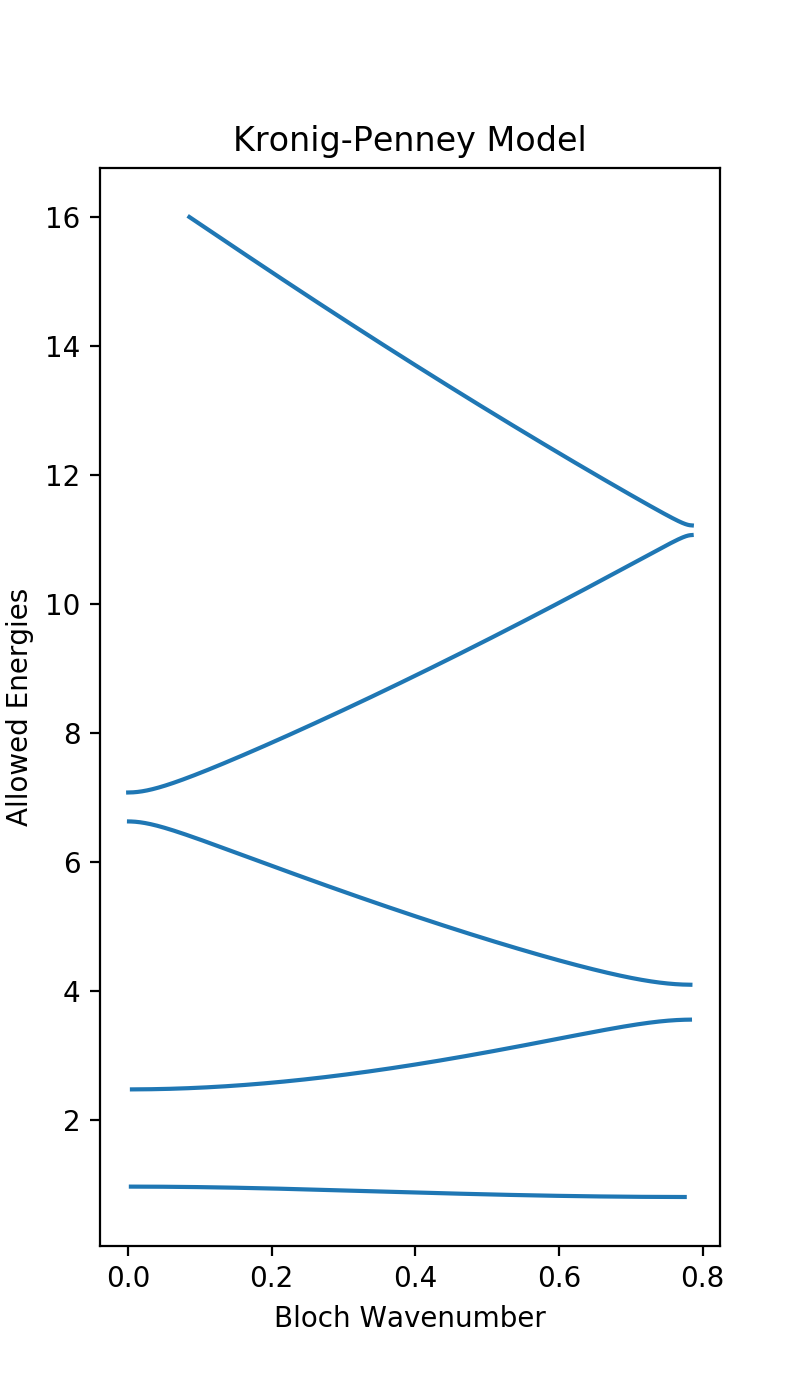
\includegraphics{plot_hw9_2c.png}
    \caption{Band Structure of the Kronig-Penney Model}
    \label{fig:band_structure_of_the_kronig_penney_model}
\end{figure}

\end{document}
